\chapter{環境}	
\thispagestyle{plain}   % chapterの直後に必ず指定

\section{Minecraftとは}\label{sec:minecraft}
Minecraftとは,創造性やサバイバル生活に焦点を当てた,サンドボックス型のゲームである.Minecraftの世界は図\ref{fig:mc_world}のように,3D空間で水平方向にほぼ無限に広がっており,木,石,土,水など様々な種類の一定の大きさの立方体ブロックで構成され,その世界にはドット絵調の動植物が存在する.プレイヤーは主に以下の二つのモードでゲームを楽しむことができる.\\

\textbf{サバイバルモード} 冒険と生活を主体としたモードである.体力や空腹度の概念が存在するため,プレイヤーは死を免れるために狩猟,採集,農業,牧畜などで食料を収集し,ブロックの収集や集めたアイテムの加工 (クラフト)を駆使して敵から逃れるための安全な住居を作らなければならない.\\

\textbf{クリエイティブモード} ブロックの組み立てに重きをおいた,創造性や実験を主体としたモードである.サバイバルモードと比較して,体力や空腹度の概念がなく,組み立てがしやすいように自由に飛行することが出来る.また,すべてのブロックを無限に配置でき,瞬時に破壊することが出来る.したがって,サバイバルモードでは制作困難な巨大建築や,複雑な回路の作成を楽しむことが出来る.\\
\begin{figure}[H]
    \centering
    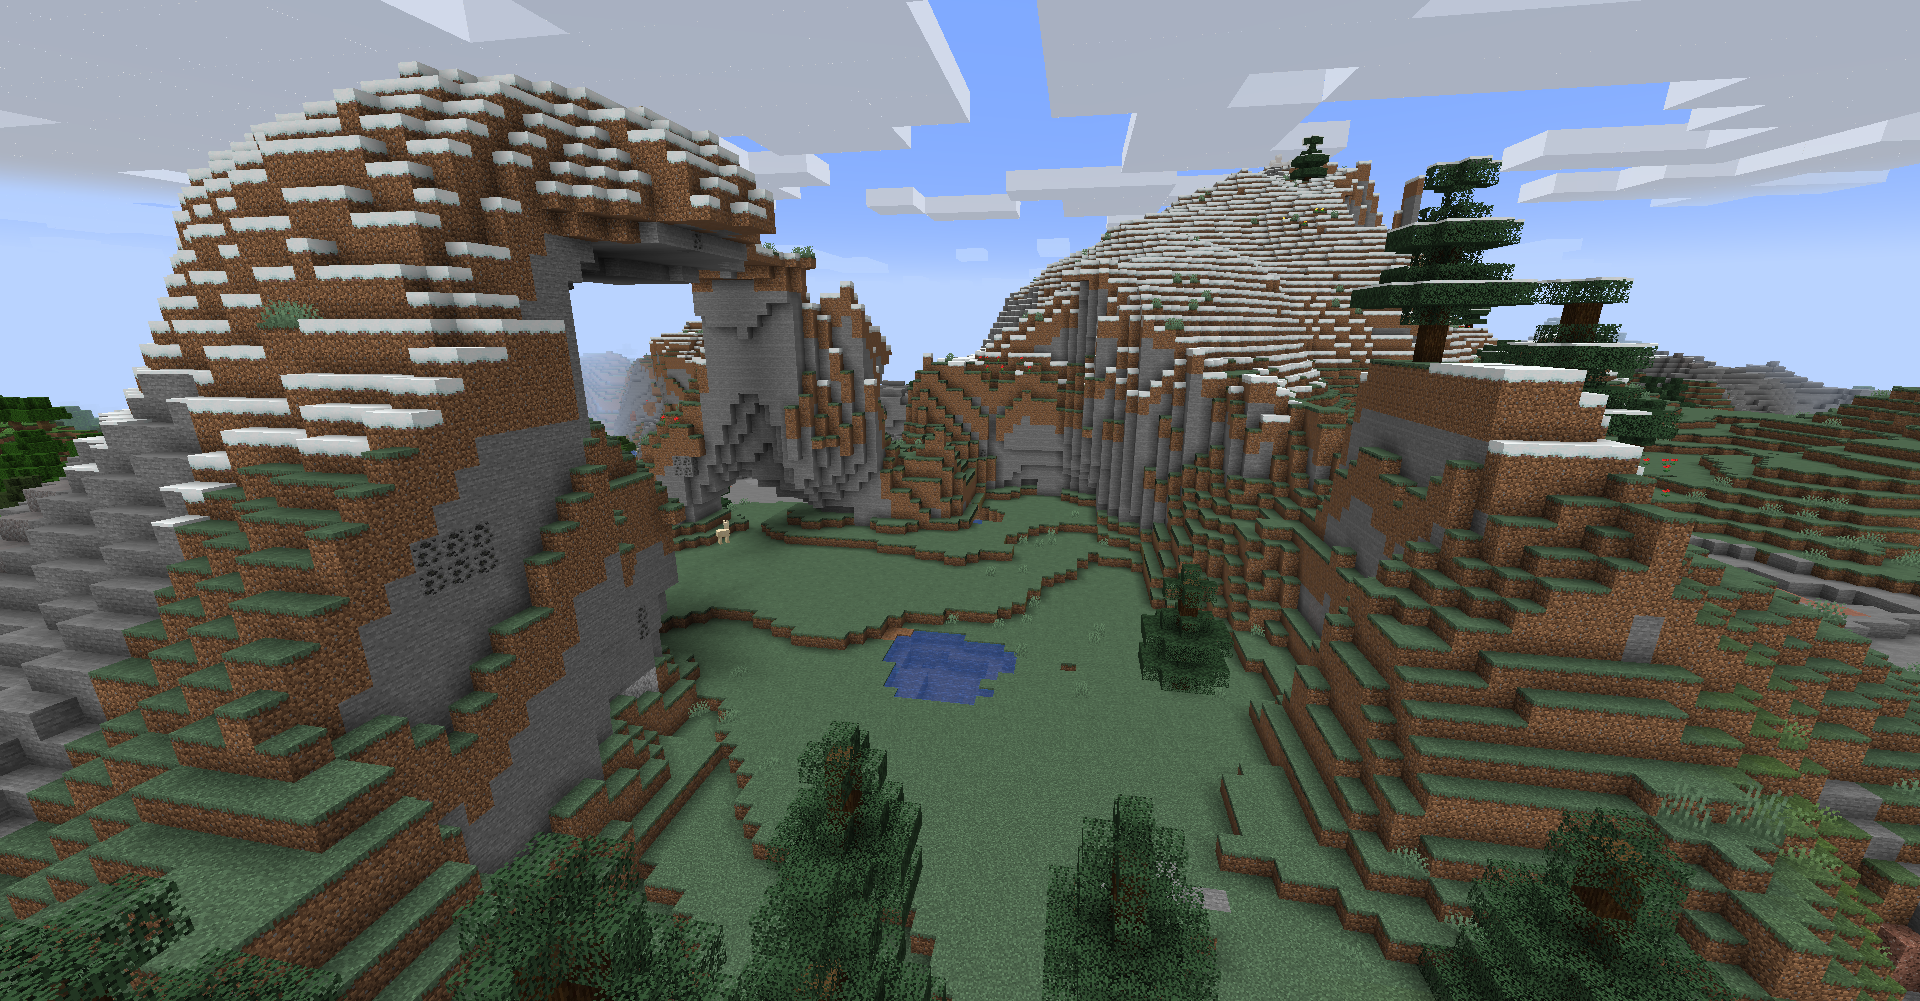
\includegraphics[width=0.7\textwidth]{fig/minecraft_world.png}
    \caption{Minecraftの世界}
    \label{fig:mc_world}
\end{figure}

\section{Minecraftの特徴}
Minecraftには,以下のような学術的に有利な特徴がある.\\

\textbf{認知度} Minecraftは2011年にPCで正式版がリリースして以来,iOSやAndroidなどのスマートフォン機種や,Xbox One,Nintendo Switchなどの家庭用ゲーム機,その他様々なプラットフォームに移植された.
また,2023年10月にはMinecraftの累計売り上げ本数が3億本を突破したことが公式ライブで発表され,世界で最も売れたインディーゲームとなった\cite{bib:minecraft_news}.
このように対応するプラットフォームが多く認知度が高いことから,ゲームのルールや特徴を知っている人が多いと予想できるため,評価実験やアンケートなどの客観的尺度が必要になった場合には遂行しやすくなることが考えられる.\\
%TODO: いつだったかの発表の好きな実況ゲームランキング入れる

\textbf{ゲーム環境} Minecraftは特定の目標がなく,オープンワールドであるため,AIの行動の可能性を広げることができる.
また,場合によってはブロックの設置によって,逆に行動を制限させることもできるので,柔軟にAIの学習環境を設定することが可能である.\\

\textbf{拡張性} Minecraftは拡張機能 (MOD) やツールの種類が多く,Minecraft最大手のMOD公開サイトとなっているCurseForgeでは,2024年1月現在で約153,204のMODプロジェクトが公開されている.
多くのMODが開発されている理由として,Minecraft EULAではMinecraftのMOD (プログラムの修正,ツール,プラグイン含む)の追加を許可しており,開発のためのコミュニティも活発であることが挙げられる.
したがって,拡張性が高いため研究に合わせてゲーム性を保ったまま自由にMinecraftをカスタムすることが出来る.\\
%TODO: Minecraft EULAのMOD推奨を入れる

\textbf{教育的価値} サバイバルや建築を楽しむことが出来るというそのゲーム性から,問題解決力や創造性を養うことが出来る.
その教育性からMinecraft公式は,Minecraft Education (教育版マインクラフト)をリリースしている. \\

\section{FUN Minecraft Serverについて}

%TODO: Minecraft Serverについて書く